\section{Benchmarking Framework}

The benchmarking framework is the same as in
Chapter~\ref{chap:benchmark-cmp}. In this section I present the benchmark
environment used to evaluate the self-indexing structures.

\subsection{Dataset}

For this benchmark we use inverted lists extracted from the Sindice dataset
from Section~\ref{sec:benchmark:framework-cmp}. Those inverted lists only
contains the entity identifiers values, the self-indexing structures being
built upon an ordered list of records, and since only the raw performance of the
self-indexing structure is measured. The other identifiers (e.g., attributes
or values identifiers) are only relevant when computing queries, thus they are
discarded for this benchmark. A small set from each frequency groups, i.e.,
HIGH, Medium and LOW groups generation presented in
Section~\ref{sec:bench-query-FW}, is extracted but keeping the entities
identifiers stream only. A list from the HIGH group will be longer than one
from the LOW group.

\subsection{Benchmark Design}

In order to have a better view of the raw performance of the self-indexing
structures, we perform two set operations, \emph{exclusion} and
\emph{conjunction}. The lists operated on are taken from one of the
three frequency groups of the Sindice dataset. Conjunction operations perform
the intersection of n lists given as operands. Exclusion operations $L_a
\backslash L_b$ exclude all the records from $L_b$ in $L_a$.

This design is based on the querying benchmark's design from the
Section~\ref{sec:bench-query-FW}. In order to process conjunctive queries, the
inverted lists from each term of the query are retrieved and intersected as
explained in Chapter~\ref{chap:IR}. To process the Boolean operator NOT,
the inverted list of the term the operator is affected to is excluded from the
results. At the core of queries processing, set operation are performed on the
retrieved lists. Based on the notation of the Section~\ref{sec:bench-query-FW},
the conjunction set operation of two inverted lists reflects the same
underlying process when computing 2-AND queries.
A measurement of the evaluation consists in the average time to execute a set
operation.

The benchmark records four information:
\begin{enumerate}
  \item the number of bytes read from the self-indexing structure.
  \item the number of documents identifiers skipped.
  \item the average time needed to perform 1 measure.
  \item the total number of search operations done on the structure as defined
  in Section~\ref{sec:cost-based-cmp}, composed of the number of
  synchronization points read plus the number of records scanned.
\end{enumerate}

The design of the SkipBlock benchmark includes two factors:
\begin{description}
\item[Operands] having two levels: HIGH-HIGH and HIGH-LOW. For instance, the
former value means that there are two operands, the HIGH and LOW inverted lists.
\item[Operation] having two levels: exclusion and conjunction.
\end{description}
Each condition of the design, i.e., HIGH-HIGH, Conjunction, possesses 100
distinct measurements.

\subsection{Implementations}

The SkipBlock model possess two implementations based on the interval search
strategies introduced in Section~\ref{sec:search-interval}. However only the S1
and S2 strategies will be discussed in these results due to a lack of time to
evaluate the others.
\begin{itemize}
  \item The baseline \emph{$I_1$} is the original Skip Lists structure with the
  linear search strategy \emph{S1}.
  \item The implementations \emph{$I_2$} and \emph{$I_3$} use respectively the
  strategies \emph{S1} and \emph{S2}. As a remainder, the S2 strategy uses
  block headers as additional synchronization points within an interval.
\end{itemize}

\section{Results}

For these benchmarks, both the self-indexing structures and the inverted list
are compressed with the VByte algorithm.
Before experimenting on the set operations, we evaluated the performance of the
self-indexing structures solely on skipping records. We first review the
evaluation results on the raw performance of the structures, before discussing
the performance with set operations.

\subsection{Advancing on a List}

In this section we evaluate the raw performance of both self-indexing models to
advance on an ordered list. The Table~\ref{tab:skipping-len} reports these
results on a list of $6\times 10^{8}$ records, records that only consist of
entity identifiers.
The first two rows reports the size in MBytes of the self-indexing structures.
A sequence of equally spaced candidates are searched,
i.e., a small skipping length of 16 and a large one of $13\times 10^{4}$
records. For each skipping length, the self-indexing structure are
parameterized with intervals of 32 and 1024, yielding for SkipBlock
respectively two possible configurations ($\vert B \vert =8, \;p=4$) and
($\vert B \vert =64, \;p=16$). 

For a same interval $\vert I \vert$ the SkipBlock structures
performs less search operations, thus saving CPU cycles as the
Table~\ref{tab:cmp-costs} have shown this aspect. However this benefit is
outweighted by the structure's size on small intervals (i.e., $\vert I \vert =
32$), since more data has to be read into memory.
Despite the predicted processing times reported in the
Table~\ref{tab:predicted-times}, the actual processing time for the SkipBlock
structure is not what was expected, i.e., half the time of the original Skip
List's. This can be explained by the compression algorithm, VByte, which is not
suited for compressing blocks.

We can note that for large skip lengths (i.e., 130 000) the SkipBlock
structures are more than 2 times as fast as the original Skip List, on large
intervals. The reason is that for so large intervals the baseline has its
number of levels considerably reduced, which is not the case for SkipBlock
since it adds in-between levels (e.g. Table~\ref{tab:skip-levels}). On top of
these additional levels, $I_3$ allow to reduce the number of search operations
by 10 times in comparison to the baseline.
When performing small skips, $I_2$ and $I_3$ implementations provide better
time than $I_1$ on large interval.

This experiment showed that the SkipBlock model provides important benefits
when jumping over a large number. With small skipping lengths, more data is
read from the SkipBlock as there are additional levels. In the latter case the
benefit of additional skipping levels is outweighted by the increased amount
of read data. We can conclude that in order to get the most benefit from
SkipBlock, configurations with large interval lengths are the most suited.

\begin{table}
\centering
\resizebox{\linewidth}{!}{%
\begin{tabular}{llc@{\hs}lllc@{\hs}lllc@{\hs}lll}
\toprule
 & $\vert I \vert$ & \phantom{a} & \multicolumn{3}{c}{$I_1$}
& \phantom{a} & \multicolumn{3}{c}{$I_2$} & \phantom{a} &
\multicolumn{3}{c}{$I_3$} \\
\cmidrule{4-6} \cmidrule{8-10} \cmidrule{12-14}
& 32 & \phantom{a} & \multicolumn{3}{c}{40.37 MB} & \phantom{a}&
\multicolumn{3}{c}{83.09 MB} & \phantom{a} & \multicolumn{3}{c}{297.57 MB} \\
& 1024 & \phantom{a} & \multicolumn{3}{c}{2.24 MB} & \phantom{a}&
\multicolumn{3}{c}{2.57 MB} & \phantom{a} & \multicolumn{3}{c}{31.6 MB} \\

\midrule
Length & & \phantom{a} & MB & Time & Ops
& \phantom{a} & MB & Time & Ops
& \phantom{a} & MB & Time & Ops \\
\multirow{2}{*}{16} & 32
&\phantom{a}& 38.11 & 12.9
s $\pm$ 135.1 ms & \numprint{338104836} 
&\phantom{a}& 59.72 & 13.8 s $\pm$ 96.8
ms & \numprint{324999973}
&\phantom{a}& 131.25 & 19.3 s $\pm$
132.1 ms & \numprint{212499973} \\
& 1024
&\phantom{a}& 2.24 & 12.6 s $\pm$ 117.7
ms & \numprint{591797454}
&\phantom{a}& 2.46 &
12.0 s $\pm$ 208.6 ms & \numprint{591250005}
&\phantom{a}& 29.28 & 14.0 s $\pm$
88.7 ms & \numprint{459999997} \\
\\
\multirow{2}{*}{\numprint{130000}} & 32
&\phantom{a}& 0.54 &
48.0 ms $\pm$ 5.8 ms & \numprint{211963}
&\phantom{a}& 0.30 & 42.3 ms $\pm$ 8.8 ms
& \numprint{109174}
&\phantom{a}& 0.31 & 47.8 ms $\pm$ 3.1 ms
& \numprint{95326} \\
& 1024
&\phantom{a}& 2.10 & 112.7 ms $\pm$
3.5 ms & \numprint{2883453}
&\phantom{a}& 0.33 & 46.1 ms $\pm$ 2.8 ms
& \numprint{2398582}
&\phantom{a}& 0.44 & 39.5 ms $\pm$ 2.1 ms
& \numprint{283796} \\
\bottomrule
\end{tabular}}
\caption{Self-indexing structures performance with equally spaced (i.e.,
$Length$) candidates. \emph{MB} stands for the number of MBytes read from the
structure. $Ops$ reports the total number of search operations performed
(i.e., the number of synchronization points read plus the number of scanned
records).}
\label{tab:skipping-len}
\end{table}

\subsection{Set Operations Results}
\label{sec:self-indexing-res}

For these benchmarks, both the self-indexing structures and the inverted list
are compressed with the VByte algorithm, so that the differences in
performance between the two structures are not caused by the compression
technique.

The performance of the self-indexing structures is compared based on the time
to perform a set operation, on the number of records that had to be scanned
from the inverted list to search for the candidates, and on the size of the
structure. We can note that the The raw results are reported in the
Table~\ref{tab:conjunction} and Table~\ref{tab:exclusion} in the appendix. For
each operands type (i.e., HIGH:HIGH or HIGH:LOW) and implementations, the best
execution time is taken and reported in the plots of the
Figure~\ref{fig:conj-excl-res}.

We observe from the plots that for either operations on two large lists (i.e.,
HIGH:HIGH type), the SkipBlock configuration of the implementation $I_3$
provides slightly better time than the original while reducing the number of
scanned records by $10^7$. However this has an impact on the structure's size
with an increase of 20 MBytes in comparison to the original model. With set
operations over lists of different sizes (i.e., LOW:HIGH type), we observe the
opposite: by scanning slightly more records and with comparable running times,
the implementation $I_3$ halves the structure's size by at least two.

For set operations on very dense lists, we are able to skip over a large number
of records with the SkipBlock model by increasing the structure's size, while
still providing similar running time as the original model. For set operations
on lists presenting a high size discrepancy, the SkipBlock model is able to
greatly reduce the structure's size while still providing similar running times.

With regards to the raw results of the Appendix~\ref{app:self-indexing:results},
this comforts the conclusion of the previous section that the SkipBlock model
provides more benefits with large intervals. We can note that the implemented
search strategies on intervals are simple ones. Thus it is possible to improve
performances by either changing the strategy, or by using an other compression
method. Indeed we used for this benchmark the VByte algorithm which is not a
block-based algorithm and thus does not profit from all the advantages of the
SkipBlock model. With a compression technique such as AFOR, we are effectively
able to reduce the size of the structure by using the frame skipping technique
(Section~\ref{sec:afor-skip}).

We can conclude that the SkipBlock model provides implementations, on large
interval lengths (e.g., 4096), that trade the structure's size cost over its
searching cost.

\begin{figure}
\centering
\resizebox{\linewidth}{!}{%
\subfloat[Two HIGH operands.] {

\begin{tikzpicture}
\begin{axis}[
        scatter/classes={
		a={mark=o},
		b={mark=star},
		c={mark=square}
% 		d={mark=diamond},
% 		e={mark=triangle}
  },
  xlabel=$Time \; (s)$,
  ylabel=$Scans$,
  mark options={scale=2},
  legend style={font=\scriptsize},
]

\addplot[red,scatter, only marks]
plot[scatter src=explicit symbolic]
coordinates {
% 	(3.400, 55766922) [a]
% 	(2.492, 55882733) [b]
% 	(2.484, 65538236) [c]
% 	(2.541, 73415418) [d]
% 	(2.619, 85376552) [e]

% 	(3.400, 50197056) [a]
% 	(2.492, 52524966) [b]
% 	(2.484, 64766407) [c]
% 	(2.541, 72983836) [d]
% 	(2.619, 85129635) [e]
	
	(2.484, 64766407) [a]
	(2.517, 72893207) [b]
	(2.582, 54730557) [c]
};

\addplot[blue,scatter, only marks]
plot[scatter src=explicit symbolic]
coordinates {
	(16.836, 54212443) [a]
	(15.826, 54205740) [b]
	(15.783, 42438570) [c]
};

% \addplot+[blue,scatter, only marks]
% plot[scatter src=explicit symbolic]
% coordinates {
% % 	(3.631, 53390244) [a]
% % 	(2.650, 54471140) [b]
% % 	(2.844, 65153966) [c]
% % 	(2.517, 73224689) [d]
% % 	(2.925, 85264977) [e]
% 	(3.631, 47270398) [a]
% 	(2.650, 51058497) [b]
% 	(2.844, 64576706) [c]
% 	(2.517, 72893207) [d]
% 	(2.925, 85080396) [e]
% };
% 
% \addplot+[green,scatter, only marks]
% plot[scatter src=explicit symbolic]
% coordinates {
% % 	(3.746, 53680730) [a]
% % 	(3.795, 53203556) [b]
% % 	(2.646, 54160474) [c]
% % 	(2.627, 56475877) [d]
% % 	(2.582, 56514322) [e]
% 	(3.746, 33665878) [a]
% 	(3.795, 42187630) [b]
% 	(2.646, 51063586) [c]
% 	(2.627, 54730109) [d]
% 	(2.582, 54730557) [e]
% };

\legend{$I_1$, $I_2$, $I_3$}
\end{axis}
\end{tikzpicture}

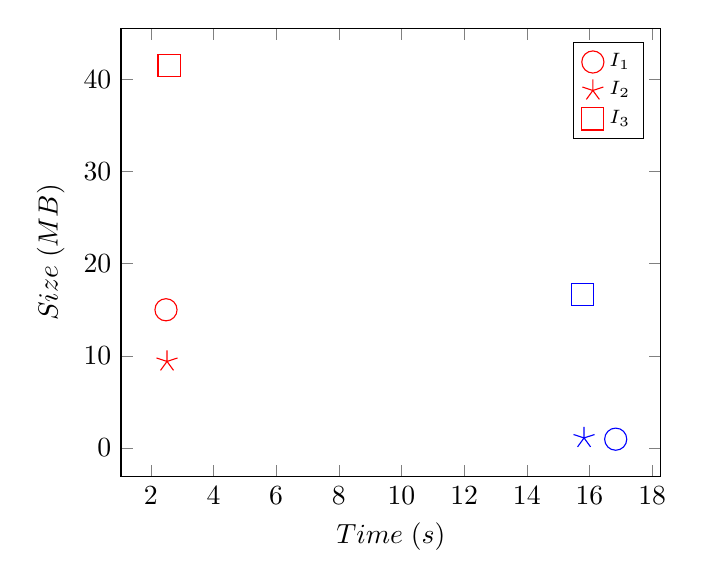
\begin{tikzpicture}
\begin{axis}[
        scatter/classes={
		a={mark=o},
		b={mark=star},
		c={mark=square}
% 		d={mark=diamond},
% 		e={mark=triangle}
  },
  xlabel=$Time \; (s)$,
  ylabel=$Size \; (MB)$,
  mark options={scale=2},
  legend style={font=\scriptsize},
  legend pos= north east
]

\addplot[red,scatter, only marks]
plot[scatter src=explicit symbolic]
coordinates {
% 	(3.400, 12.02) [a]
% 	(2.492, 7.36) [b]
% 	(2.484, 2.97) [c]
% 	(2.541, 1.66) [d]
% 	(2.619, 0.95) [e]
	
	(2.484, 15) [a]
	(2.517, 9.39) [b]
	(2.582, 41.53) [c]
};

\addplot[blue,scatter, only marks]
plot[scatter src=explicit symbolic]
coordinates {
	(16.836, 0.941) [a]
	(15.826, 1.076) [b]
	(15.783, 16.69) [c]
};

% \addplot+[blue,scatter, only marks]
% plot[scatter src=explicit symbolic]
% coordinates {
% 	(3.631, 14.10) [a]
% 	(2.650, 9.16) [b]
% 	(2.844, 2.25) [c]
% 	(2.517, 1.30) [d]
% 	(2.925, 0.74) [e]
% };
% 
% \addplot+[green,scatter, only marks]
% plot[scatter src=explicit symbolic]
% coordinates {
% 	(3.746, 40.83) [a]
% 	(3.795, 23.87) [b]
% 	(2.646, 7.60) [c]
% 	(2.627, 4.99) [d]
% 	(2.582, 4.81) [e]
% };

\legend{$I_1$, $I_2$, $I_3$}
\end{axis}
\end{tikzpicture}


}}\quad
\resizebox{\linewidth}{!}{%
\subfloat[Two operands, one HIGH and one LOW.] {

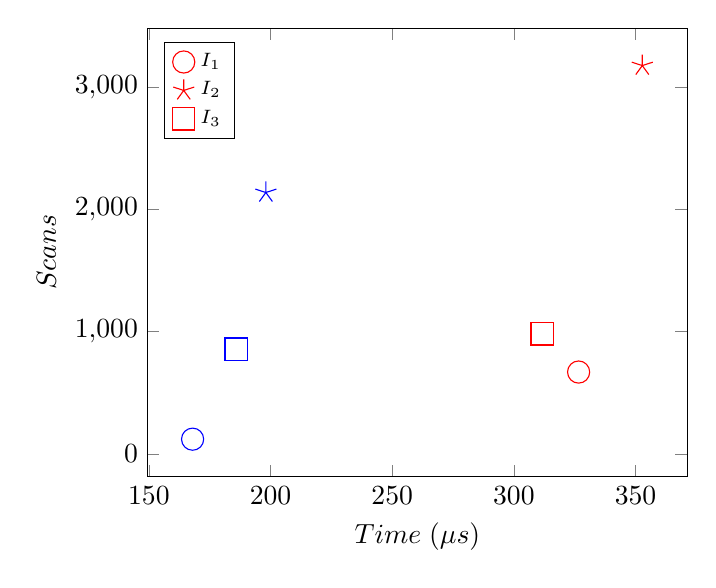
\begin{tikzpicture}
\begin{axis}[
        scatter/classes={
		a={mark=o},
		b={mark=star},
		c={mark=square}
% 		d={mark=diamond},
%  		e={mark=triangle}
  },
  xlabel=$Time \; (\mu s)$,
  ylabel=$Scans$,
  mark options={scale=2},
  legend style={font=\scriptsize},
  legend pos= north west
]

\addplot[red,scatter, only marks]
plot[scatter src=explicit symbolic]
coordinates {
% 	(363.501, 1398) [a]
% 	(326.611, 2088) [b]
% 	(545.605, 9659) [c]
% 	(579.102, 13397) [d]
% 	(735.205, 24296) [e]

% 	(363.501, 447) [a]
% 	(326.611, 670) [b]
% 	(545.605, 4315) [c]
% 	(579.102, 8407) [d]
% 	(735.205, 16207) [e]

	(326.611, 670) [a]
	(352.783, 3176) [b]
	(311.572, 982) [c]
};

\addplot[blue,scatter, only marks]
plot[scatter src=explicit symbolic]
coordinates {
	(167.969, 121) [a]
	(198.083, 2138) [b]
	(185.840, 858) [c]
};

% \addplot+[blue,scatter, only marks]
% plot[scatter src=explicit symbolic]
% coordinates {
% % 	(581.592, 932) [a]
% % 	(521.191, 990) [b]
% % 	(352.783, 3176) [c]
% % 	(432.813, 5718) [d]
% % 	(453.247, 8605) [e]
% 	(581.592, 329) [a]
% 	(521.191, 489) [b]
% 	(352.783, 2733) [c]
% 	(432.813, 5292) [d]
% 	(453.247, 8100) [e]
% };
% 
% \addplot+[green,scatter, only marks]
% plot[scatter src=explicit symbolic]
% coordinates {
% % 	(640.820, 862) [a]
% % 	(585.107, 820) [b]
% % 	(381.714, 1102) [c]
% % 	(370.581, 1539) [d]
% % 	(311.572, 1739) [e]
% 	(640.820, 150) [a]
% 	(585.107, 234) [b]
% 	(381.714, 521) [c]
% 	(370.581, 982) [d]
% 	(311.572, 982) [e]
% };

% \legend{16, 32, 256, 512, 1024}
\legend{$I_1$, $I_2$, $I_3$}
\end{axis}
\end{tikzpicture}

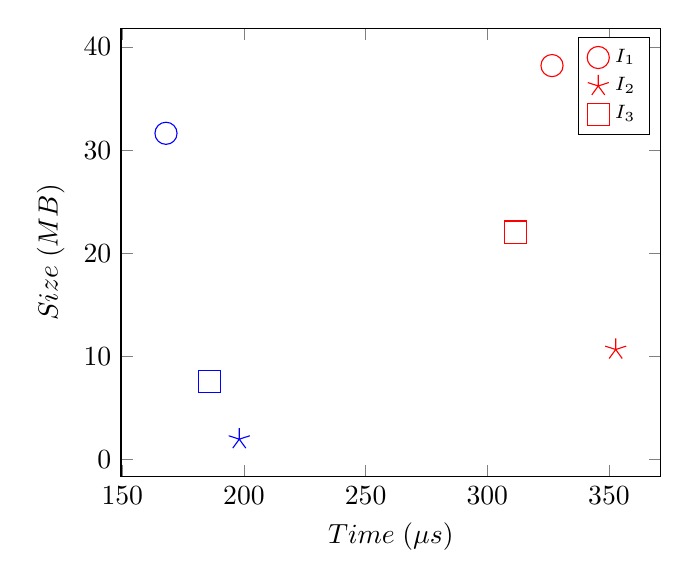
\begin{tikzpicture}
\begin{axis}[
        scatter/classes={
		a={mark=o},
		b={mark=star},
		c={mark=square}
% 		d={mark=diamond},
%  		e={mark=triangle}
  },
  xlabel=$Time \; (\mu s)$,
  ylabel=$Size \; (MB)$,
  mark options={scale=2},
  legend style={font=\scriptsize},
%   legend pos= north west
]

\addplot[red,scatter, only marks]
plot[scatter src=explicit symbolic]
coordinates {
% 	(363.501, 0.004) [a]
% 	(326.611, 0.006) [b]
% 	(545.605, 0.024) [c]
% 	(579.102, 0.022) [d]
% 	(735.205, 0.032) [e]
	
	(326.611, 38.2) [a]
	(352.783, 10.65) [b]
	(311.572, 22.05) [c]
};

\addplot[blue,scatter, only marks]
plot[scatter src=explicit symbolic]
coordinates {	
	(167.969, 31.63) [a]
	(198.083, 1.95) [b]
	(185.840, 7.57) [c]
};

% \addplot+[blue,scatter, only marks]
% plot[scatter src=explicit symbolic]
% coordinates {
% 	(581.592, 0.0031) [a]
% 	(521.191, 0.0026) [b]
% 	(352.783, 0.0023) [c]
% 	(432.813, 0.0023) [d]
% 	(453.247, 0.0027) [e]
% };
% 
% \addplot+[green,scatter, only marks]
% plot[scatter src=explicit symbolic]
% coordinates {
% 	(640.820, 0.0034) [a]
% 	(585.107, 0.0028) [b]
% 	(381.714, 0.0027) [c]
% 	(370.581, 0.0027) [d]
% 	(311.572, 0.0034) [e]
% };

\legend{$I_1$, $I_2$, $I_3$}
\end{axis}
\end{tikzpicture}
}}
\caption{Conjunction (in red) and exclusion (in blue) set operations. The time
on the x axis is the best average time, from the
Appendix~\ref{app:self-indexing:results}, to perform the operation on the
given operands for an implementation.}
\label{fig:conj-excl-res}
\end{figure}
